\section{Intro to Matrices}

\paragraph{
    In mathematics, a matrix (plural: matrices) is a grid of elements. You can think of a matrix as being like a 2D array. For example:
}

\paragraph{
    \begin{equation*}
    \begin{pmatrix}
    2 & 1\\
    0 & 3
    \end{pmatrix}
    \end{equation*}
}

\paragraph{
    Just like vectors, matrices can be of any size, but only sizes from 1 to 4 are used. Matrices are named based on their dimensions; a matrix that is 3 elements wide and 2 elements tall would be a 3x2 matrix. In computing, when the height and width are the same, it is common to abbreviate it to just the one number; a 4x4 matrix is just called a mat4 in GLM.
}

\paragraph{
    You can create a matrix in GLM as follows:
}

\begin{frame}{}
    \begin{figure}[ht]
    \centering
    \colorbox{backgroundcolor}{
        \parbox{0.9\textwidth}{
            \lstinputlisting[language=csh,style=csharp]
            {code/chap2_MathematicsPrinciples/CreatingAMatrix.cpp}
        }
    }
    \caption{Creating a matrix}
    \label{fig:creating_a_matrix}
    \end{figure}
\end{frame}

\paragraph{
    Matrices are very important for graphics programming; matrices are how you can move around your polygons without having to replace their vertices. Scaling, translation, and rotation are all accomplished using matrices.
}

\subsection{Row Major vs Column Major}
\paragraph{
    Before you can learn anything about matrices, you need to understand matrix ordering.
}

\paragraph{
    There is some debate as to how matrices should be laid out in memory. Matrices are made up of rows (horizontal) and columns (vertical). There are two different ways a matrix can be laid out: row-major, and column-major.
}

\paragraph{
    In row-major, the index progresses from left to right, dropping down to the next row after reaching the end. In column-major matrices, the index progresses from top to bottom, moving right to the next column after reaching the end. To demonstrate:
}

\begin{frame}{}
    \begin{figure}[ht]
      \centering
      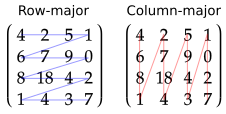
\includegraphics[width=0.5\textwidth]{images/chap2/RowVsColumn.png}
      \caption{Row-major vs column-major matrix ordering}
      \label{fig:row_vs_column}
    \end{figure}
\end{frame}

\paragraph{
    In this example, if you looked at the fifth element, you'd see 6 if you were using row-major, or 2 if you're using column major.
}

\paragraph{
    GLM uses row-major for all operations, so this book will as well. \emph{If you run into unexpected behavior while using matrices, it could be because you're using column-major instead}.
}

\paragraph{
    Luckily, converting between row-major and column-major (and vice-versa) is very simple. The process is known as \emph{transposing}. If you get incorrect results from a matrix operation, transposing should be your first debugging step. You can transpose a matrix in GLM as follows:
}

\begin{frame}{}
    \begin{figure}[ht]
    \centering
    \colorbox{backgroundcolor}{
        \parbox{0.9\textwidth}{
            \lstinputlisting[language=csh,style=csharp]
            {code/chap2_MathematicsPrinciples/TransposingAMatrix.cpp}
        }
    }
    \caption{Creating a matrix}
    \label{fig:creating_a_matrix}
    \end{figure}
\end{frame}

\subsection{Matrix addition and subtraction}
\paragraph{
    Like vectors, matrix addition and subtraction are both done component-wise:
}

\paragraph{
    \begin{equation*}
    \begin{pmatrix}
    2 & 1\\
    0 & 3
    \end{pmatrix} +\begin{pmatrix}
    8 & 7\\
    4 & 9
    \end{pmatrix} =\begin{pmatrix}
    2+8 & 1+8\\
    0+4 & 3+9
    \end{pmatrix} =\begin{pmatrix}
    10 & 9\\
    4 & 12
    \end{pmatrix}
    \end{equation*}
}

\paragraph{
    Scalar operations also still work the same way:
}

\paragraph{
    \begin{equation*}
    \begin{pmatrix}
    2 & 1\\
    0 & 3
    \end{pmatrix} +7=\begin{pmatrix}
    2+7 & 1+7\\
    0+7 & 3+7
    \end{pmatrix} =\begin{pmatrix}
    9 & 8\\
    7 & 10
    \end{pmatrix}
    \end{equation*}
}

\subsection{Matrix multiplication}
\paragraph{
    Matrices can be multiplied by a scalar the same way vectors can:
}

\paragraph{
    \begin{equation*}
    \begin{pmatrix}
    2 & 1\\
    0 & 3
    \end{pmatrix} \times 3=\begin{pmatrix}
    2\times 3 & 1\times 3\\
    0\times 3 & 3\times 3
    \end{pmatrix} =\begin{pmatrix}
    6 & 3\\
    0 & 9
    \end{pmatrix}
    \end{equation*}
}

\paragraph{
    Multiplication with a vector or another matrix is where matrices become more difficult, but also more useful. Like with vectors, component-wise matrix multiplication isn't possible. Unlike vectors, the dot product and cross product are not defined for matrices.
}